\documentclass[Royal,times,sageh]{sagej}

\usepackage{moreverb,url,natbib, multirow, tabularx}
\usepackage[colorlinks,bookmarksopen,bookmarksnumbered,citecolor=red,urlcolor=red]{hyperref}





\begin{document}

\title{Missing the Point: Non-Convergence in Iterative Imputation Algorithms}

\runninghead{Oberman}

\author{H. I. Oberman\affilnum{1}}

\affiliation{\affilnum{1}{Department of Methodology and Statistics, Utrecht University, Utrecht, The Netherlands.}}

\corrauth{Hanne Oberman, Sjoerd Groenman building, Padualaan 14, 3584 CH, Utrecht, The Netherlands.}

\email{\href{mailto:h.i.oberman@uu.nl}{\nolinkurl{h.i.oberman@uu.nl}}}

\begin{abstract}
Iterative imputation is a popular tool to accommodate missing data. While it is widely accepted that valid inferences can be obtained with this technique, these inferences all rely on algorithmic convergence. There is no consensus on how to evaluate the convergence properties of the method. This paper provides insight into identifying non-convergence in iterative imputation algorithms. Our study found that---in the cases considered---inferential validity was achieved after five to ten iterations, much earlier than indicated by the \(\widehat{R}\) and \(AC\) diagnostics. We conclude that it never hurts to iterate longer, but such calculations hardly bring added value.
\end{abstract}

\keywords{missing data, iterative imputation, non-convergence, MICE}

\maketitle

\hypertarget{introduction}{%
\section{Introduction}\label{introduction}}

Anyone who analyzes person-data may run into a missing data problem. Missing data is not only ubiquitous across science, but treating it can also be a tedious task. If a dataset contains just one incomplete observation, calculations are not defined, and statistical models cannot be fitted to the data. To circumvent this, many statistical packages employ list-wise deletion by default (i.e., ignoring incomplete observations). Unfortunately, this \emph{ad hoc} solution may yield invalid results \citep{buur18}. An alternative is to apply imputation. With imputation, we `fill in' the missing values in an incomplete dataset. Subsequently, the model of scientific interest can be fitted to the completed dataset. By repeating this process several times, a distribution of plausible results may be obtained, which reflects the uncertainty in the data due to missingness. This technique is known as `multiple imputation' \citep[MI;][]{rubin76}. MI has proven to be a powerful tool to draw valid inferences from incomplete data under many circumstances \citep{buur18}.

Figure \ref{fig:diagram} provides an overview of the steps involved with MI. The missing part \(y_{\rm mis}\) of an incomplete dataset is imputed \(m\) times. This creates \(m\) sets of imputed data \(\dot y_{\rm imp, \ell}\), where \(\ell = 1, 2, ..., m\). The imputed data is then combined with the observed data \(y_{\rm obs}\) to create \(m\) completed datasets. On each of these datasets the analysis of scientific interest is performed to estimate \(Q\): the quantity of scientific interest (e.g., a regression coefficient). Since \(Q\) is estimated on each completed dataset, \(m\) separate \(\hat{Q}_\ell\)-values are obtained. Finally, the \(\hat{Q}_\ell\)-values are combined into a single pooled estimate \(\bar{Q}\). The premise of multiple imputation is that \(\bar{Q}\) is an unbiased and confidence-valid estimate of the true---but unobserved---scientific estimand \(Q\) \citep{rubin96}.

\begin{figure}

{\centering 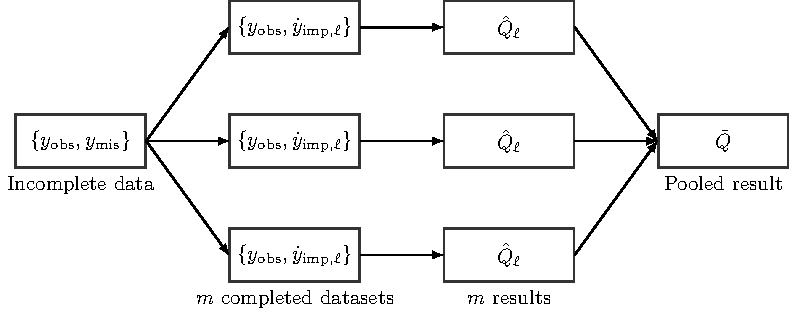
\includegraphics[width=\linewidth]{../Figures/DiagramMI} 

}

\caption{Scheme of the main steps in multiple imputation---from an incomplete dataset, to $m=3$ multiply imputed datasets, to $m=3$ estimated quantities of scientific interest $\hat{Q}$, to a single pooled estimate $\bar{Q}$.}\label{fig:diagram}
\end{figure}

A popular method to obtain imputations is to use the `Multiple Imputation by Chained Equations' algorithm, shorthand `MICE'\citep{mice}. With MICE, imputed values are drawn from the posterior predictive distribution of the missing values. The algorithm is named after its iterative nature: a multivariate distribution is obtained by iterating over a sequence of univariate imputations. Iteration, however, also introduces a potential threat to the validity of the imputations: What if the algorithm has not converged? Are the imputations then to be trusted? And can we rely on the inference obtained on the completed data?

These remain open questions since the convergence properties of iterative imputation algorithms have not been systematically studied \citep{buur18}. There is no scientific consensus on how to evaluate the convergence of imputation algorithms \citep{zhu15, taka17}. Moreover, the behavior of such algorithms under certain default imputation models (e.g., `predictive mean matching') is an entirely open question \citep{murr18}. Therefore, algorithmic convergence should be monitored carefully---although this is not straightforward. Iterative imputation algorithms such as MICE are special cases of Markov chain Monte Carlo (MCMC) methods. In MCMC methods, convergence is not from a scalar to a point, but from one distribution to another. The values generated by the algorithm (e.g., imputed values) will vary even after convergence \citep{gelm13}. Since MCMC algorithms do not reach a unique point at which convergence is established, diagnostic methods may only identify signs of \emph{non}-convergence \citep{hoff09}. Several non-convergence diagnostics exist, but it is not known whether these are appropriate within the imputation framework.

In this paper we study different methods for assessing non-convergence in iterative imputation algorithms. We define several diagnostics and evaluate how these diagnostics could be appropriate for iterative imputation applications. We then address the impact of inducing non-convergence in iterative imputation algorithms through model-based simulation in \texttt{R} \citep{R}. For reasons of brevity, we only focus on the iterative imputation algorithm implemented in the popular \texttt{mice} package in \texttt{R} \citep{mice}. The aim of the simulation study is to determine whether unbiased, confidence-valid inferences may be obtained if the algorithm has not (yet) converged. And additionally, to evaluate the behavior and performance of several diagnostic methods to identify non-convergence. With that, we formulate an informed advice on when it is safe to conclude that the algorithm is converged \emph{enough} for valid inferences. We translate the results of the study into guidelines for applied researchers, which may facilitate drawing valid inferences from incomplete data.

\hypertarget{some-notation}{%
\subsection{Some notation}\label{some-notation}}

Let \(y\) denote an \(n \times k\) matrix containing the data values on \(k\) variables for all \(n\) units in a sample. The data value of unit \(i\) (\(i = 1, 2, \dots, n\)) on variable \(j\) (\(j = 1, 2, \dots, k\)) may be either observed or missing. The number of units \(i\) with at least one missing value, divided by the total number of units \(n\), is called the proportion of incomplete cases \(p_{\rm inc}\) in dataset \(y\). The collection of observed data values in \(y\) is denoted by \(y_{\rm obs}\); the missing part of \(y\) is referred to as \(y_{\rm mis}\). For each datapoint in \(y_{\rm mis}\), we sample \(m \times T\) plausible values, where \(m\) is the number of imputations (\(\ell = 1, 2, \dots, m\)) and \(T\) is the number of iterations in the imputation algorithm (\(t = 1, 2, \dots, T\)). The state-space of the algorithm at a certain iteration \(t\) may be summarized by a scalar summary \(\theta\) (e.g., the average of the imputed values). The collection of \(\theta\)-values between \(t=1\) (summarizing the state-space of the algorithm at initialization) and \(t=T\) (summarizing the state-space for the imputed values) will be referred to as an `imputation chain'.

\hypertarget{algorithmic-non-convergence}{%
\section{Algorithmic non-convergence}\label{algorithmic-non-convergence}}

There are two requirements for convergence of iterative algorithms: mixing and stationarity \citep{gelm13}. In iterative imputation algorithms, mixing implies that imputation chains intermingle nicely, and stationarity is characterized by the absence of trending across iterations. If one of the two requirements is not met, we speak of non-convergence. Without mixing, chains may be `stuck' at a local optimum, instead of sampling imputed values from the entire predictive posterior distribution of the missing values. The distribution of imputed values then differs across imputations. This may cause under-estimation of the variance between chains, which results in spurious, invalid inferences. Without stationarity, there is trending within imputation chains. Trending implies that further iterations would yield a systematically lower or higher set of imputations. Iterative imputation algorithms that have not (yet) reached stationarity, may thus yield biased estimates.

To illustrate what non-mixing and non-stationarity look like in iterative imputation algorithms, we reproduce an example from van Buuren \citeyearpar[\(\S\) 6.5.2]{buur18}. Figure \ref{fig:non-conv} displays two scenarios from the example. The panel on the left-hand side of the figure shows typical convergence of an iterative imputation algorithm. The right-hand side displays pathological non-convergence, induced by purposefully mis-specifying the imputation model. Each line portrays one imputation chain (i.e., the values of a scalar summary \(\theta\) across iterations). The \(\theta\) depicted here is the `chain mean' of variable \(j\), which is defined as the average of variable \(j\) in the \(m\) sets of imputations \(\dot y_{\rm imp, \ell}\).

In the typical convergence scenario, the imputation chains intermingle nicely and there is little to no trending. In the non-convergence scenario, there is a lot of trending and some chains do not intermingle. Importantly, the chain means at the last iteration (the imputed values per imputation \(\ell\)) are very different between the two scenarios. The algorithm with the mis-specified model yields imputed values that are on average a factor two larger than those of the typically converged algorithm. It is obvious that non-convergence in this example impacts the distribution of the imputed values per imputation \(\dot y_{\rm imp, \ell}\). This effect may translate into the distribution of the \(m\) sets of completed data \{\(y_{\rm obs}, \dot y_{\rm imp, \ell}\)\}, which consequently affects the estimated quantities of scientific interest \(\hat{Q}_{\ell}\), and finally the pooled estimate \(\bar{Q}\). \(\bar{Q}\) is then a biased, invalid estimate of \(Q\). Therefore, it is important to reach algorithmic convergence in iterative imputation algorithms.

\begin{figure}

{\centering 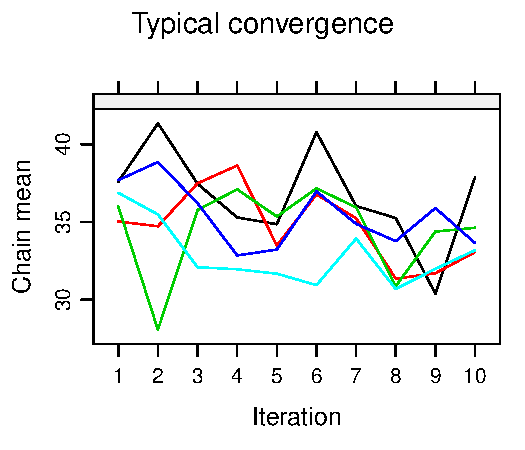
\includegraphics[width=.49\linewidth]{2.Manuscript_files/figure-latex/non-conv-1} 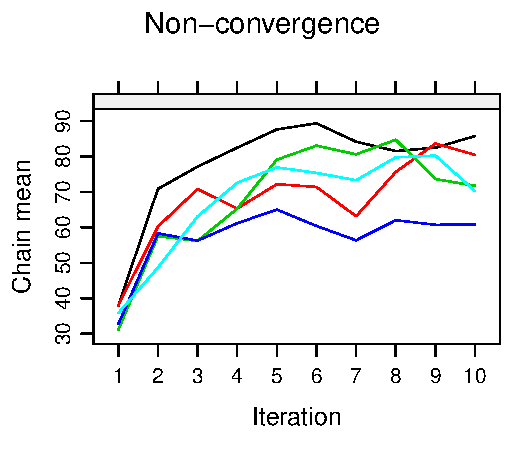
\includegraphics[width=.49\linewidth]{2.Manuscript_files/figure-latex/non-conv-2} 

}

\caption{Typical convergence versus pathological non-convergence (reproduced from van Buuren; 2018). Depicted are chain means of variable $j$ in each imputation ($m=5$; $T=10$). Please note that any difference between the two scenarios (see e.g., the magnitude of the chain means on the y-axes) stems from the imputation algorithms---the two scenarios have equal incomplete data $y$.}\label{fig:non-conv}
\end{figure}

\hypertarget{identifying-non-convergence}{%
\subsection{Identifying non-convergence}\label{identifying-non-convergence}}

Currently, the recommended practice for evaluating the convergence of the MICE algorithm is through visual inspection. After running the imputation algorithm for a certain number of iterations, researchers are encouraged to produce traceplots. In a traceplot, a scalar summary of the state-space of the algorithm \(\theta\) is plotted against the iteration number, as depicted in Figure \ref{fig:non-conv}. The default scalar summaries to inspect for the MICE algorithm are chain means and chain variances. Non-convergence is diagnosed if the imputation chains are not freely intermingled with one another, or if the chains show definite trends \citep[\(\S\) 6.5.2]{buur18}.

Identifying non-convergence by inspecting traceplots may be undesirable for several reasons: 1) it may be challenging to the untrained eye, 2) only severely pathological cases of non-convergence may be diagnosed, and 3) there is not an objective measure that quantifies convergence \citep[\(\S\) 6.5.2]{buur18}. Moreover, traceplots are typically only used to inspect univariate \(\theta\)s. Monitoring univariate summaries of the state-space of the algorithm may be insufficient because MICE is not only concerned with a single column, but the entire multivariate distribution of the imputations. Ideally, we would monitor a multivariate \(\theta\).

A suggestion by \citet{buur18} for a multivariate \(\theta\) to monitor is the estimated quantity of scientific interest \(\hat{Q}\), which usually is multivariate in nature. This \(\theta\) is computed as the estimate in each imputation, \(\hat{Q}_\ell\), across iterations. Implementing this, however, might be somewhat too technical for empirical researchers. Besides, this scalar summary is not model-independent. That is, \(\theta=\hat{Q}\) is not universal to all complete data problems, while one of the advantages of iterative imputation is that the missing data problem and scientific problem are solved independently. Focusing on the convergence of outcome parameters may influence the iterative imputation procedure in the sense that the model of evaluation favors the model of interest. On these grounds, such a \(\theta\) can be considered insufficient too.

As alternative, van Buuren \citeyearpar[\(\S\) 4.5.2]{buur18} proposed multivariate evaluation of the MICE algorithm through eigenvalue decomposition, building on the work of \citet{mack03}. This technique may yield a model-independent, multivariate scalar summary to monitor, but it is not implemented in the \texttt{mice} package \citep{mice}.

\hypertarget{a-novel-scalar-summary}{%
\subsection{A novel scalar summary}\label{a-novel-scalar-summary}}

To monitor non-convergence in iterative imputation algorithms, we may summarize the state-space of the algorithm with several \(\theta\)s. The downside to the current \(\theta\)s is that they either focus on the univariate state-space, or primarily track the change over the iterations of a multivariate outcome conform the scientific model of interest. Ideally, one would like to evaluate a model-independent \(\theta\) that summarizes the multivariate nature of the data.

We propose \(\lambda_{1}\) as such a scalar summary. We define \(\lambda_{1}\) as the first eigenvalue of the variance-covariance matrix in the \(m\) completed datasets. The eigenvalues of a variance-covariance matrix \(S\) summarize the total set of covariances in the data. Let \(\lambda_{1, \ell} \geq \lambda_{2, \ell} \geq ... \geq \lambda_{j, \ell}\) be the eigenvalues of \(S_\ell\) in each imputation. The first eigenvalue, \(\lambda_{1,\ell}\), then summarizes the largest possible amount of covariance in each completed dataset \{\(y_{\rm obs}, \dot y_{\rm imp, \ell}\)\}. By definition, \(\lambda_{1}\)-values are equal to the variance of the first component that would be obtained by performing principal component analysis (PCA) on the completed data. As scalar summary, \(\lambda_{1}\) has the appealing property that it is not dependent on the model of scientific interest, yet still summarizes the multivariate state-space of the algorithm.

In this study, we consider each of the four \(\theta\)s that we discussed. Namely, two univariate scalar summaries (chain mean and chain variance), a model-dependent multivariate summary \(\hat{Q}\), and the novel model-independent multivariate summary \(\lambda_1\).

\hypertarget{non-convergence-diagnostics}{%
\section{Non-convergence diagnostics}\label{non-convergence-diagnostics}}

There are many diagnostic tools to identify non-convergence in iterative (MCMC) algorithms \citep{broo98, elad06}. We consider only two of them that may be appropriate for imputation algorithms---one to monitor signs of non-mixing, and one for non-stationarity. As recommended by e.g.~\citet{cowl96} we will use the potential scale reduction factor \(\widehat{R}\) to evaluate mixing \citep[`Gelman-Rubin statistic';][]{gelm92}, and autocorrelation to diagnose trending \citep[\(AC\);][]{scha97, gelm13}. With a recently proposed adaptation, \(\widehat{R}\) might also serve to diagnose non-stationarity, but this has not yet been thoroughly investigated \citep{veht19}. Therefore, we will evaluate the appropriateness of both \(\widehat{R}\) versions, in addition to \(AC\). Other methods are outside the scope of this study because they e.g.~assume that values within chains represent independent samples, whereas the MICE algorithm only uses the final iteration to produce imputations.

\hypertarget{potential-scale-reduction-factor}{%
\subsection{Potential scale reduction factor}\label{potential-scale-reduction-factor}}

In 2019, Vehtari et al.~proposed an updated version of the potential scale reduction factor \(\widehat{R}\), originally coined in 1992. The adapted version would be better suited to detect non-mixing in the tails of distributions, and even identify non-stationarity. This version uses three transformations on the scalar summary \(\theta\), before computing \(\widehat{R}\)-values. Namely, rank-normalization, folding, and localization. The definition of the diagnostic itself is equal to the original \(\widehat{R}\). Therefore, we may follow Vehtari et al.'s formulation (2019, p.~5) to define both \(\widehat{R}\) versions. Let \(m\) be the total number of chains, \(T\) the number of iterations per chain (where \(T\geq2\)), and \(\theta\) the scalar summary of interest. For each chain (\(\ell = 1, 2, \dots, m\)), we estimate the variance of \(\theta\), and average these to obtain within-chain variance \(W\).

\begin{align*}
W&=\frac{1}{m} \sum_{\ell=1}^{m} s_{\ell}^{2}, \text { where } s_{\ell}^{2}=\frac{1}{T-1} \sum_{t=1}^{T}\left(\theta^{(t \ell)}-\bar{\theta}^{(\cdot \ell)}\right)^{2}. 
\end{align*}

\noindent We then estimate between-chain variance \(B\) (note that we diverge from the typical notation in MI, where \(B\) denotes the variance between the estimated quantities of scientific interest \(\hat{Q}_{\ell}\)). \(B\) is defined as the variance of the collection of average \(\theta\)s per chain:

\begin{align*}
B&=\frac{T}{m-1} \sum_{\ell=1}^{m}\left(\bar{\theta}^{(\cdot \ell)}-\bar{\theta}^{(\cdot \cdot)}\right)^{2}, \text { where } \bar{\theta}^{(\cdot \ell)}=\frac{1}{T} \sum_{t=1}^{T} \theta^{(t \ell)} \text{, } \bar{\theta}^{(\cdot \cdot)}=\frac{1}{m} \sum_{\ell=1}^{m} \bar{\theta}^{(\cdot \ell)}. 
\end{align*}

\noindent From the between- and within-chain variances we compute a weighted average, \(\widehat{\operatorname{var}}^{+}\), which over-estimates the total variance of \(\theta\). \(\widehat{R}\) is then obtained as a ratio between this total variance and the within-chain variance:

\begin{equation*}
\widehat{R}=\sqrt{\frac{\widehat{\operatorname{var}}^{+}(\theta | y)}{W}},
\text{ where } \widehat{\operatorname{var}}^{+}(\theta | y)=\frac{T-1}{T} W+\frac{1}{T} B.
\end{equation*}

We can interpret \(\widehat{R}\) as potential scale reduction factor since it indicates by how much the variance of \(\theta\) could be shrunken down if an infinite number of iterations per chain would be run \citep{gelm92}. The assumption underlying this interpretation is that chains are `over-dispersed' at \(t=1\), and reach convergence as \(T \to \infty\). Over-dispersion implies that the initial values of the chains are `far away' from the target distribution and each other. When the sampled values in each chain are independent of the chain's initial value, the mixing component of convergence is satisfied. The variance between chains, \(B\), is then equivalent to the variance within chains, \(W\), and \(\widehat{R}\)-values will be close to one. High \(\widehat{R}\)-values thus indicate non-convergence.

\hypertarget{autocorrelation}{%
\subsection{Autocorrelation}\label{autocorrelation}}

Autocorrelation is defined as the correlation between two subsequent \(\theta\)-values within the same chain \citep[p.~147]{lync07}. In this study, we only consider \(AC\) at lag 1, i.e., the correlation between the \(t^{th}\) and \((t+1)^{th}\) iteration of the same chain. Following the same notation as for \(\widehat{R}\),

\begin{equation*}
AC = \left( \frac{T}{T-1} \right) \frac{\sum_{t=1}^{T-1}(\theta_t - \bar{\theta}^{(\cdot m)})(\theta_{t+1} - \bar{\theta}^{(\cdot m)})}{\sum_{t=1}^{T}(\theta_t - \bar{\theta}^{(\cdot m)})^2}.
\end{equation*}

We can interpret \(AC\)-values as a measure of non-stationarity. If there is dependence between subsequent \(\theta\)-values in imputation chains, \(AC\)-values are non-zero. Positive \(AC\)-values occur when \(\theta\)-values are recurring (i.e., high \(\theta\)-values are followed by high \(\theta\)-values, and low \(\theta\)-values are followed by low \(\theta\)-values). Recurrence within imputation chains may lead to trending. Negative \(AC\)-values occur when \(\theta\)-values of subsequent iterations are less similar, or diverge from one another. Divergence within imputation poses no threat to the convergence of the algorithm---it may even speed up convergence. Complete stationarity is reached when \(AC=0\). As non-convergence diagnostic, our interest is in positive \(AC\)-values.

\hypertarget{thresholds}{%
\subsection{Thresholds}\label{thresholds}}

It is unlikely that iterative algorithms such as MICE will achieve the ideal values of \(\widehat{R}=1\) and \(AC=0\). Because of its convergence to a distribution, the algorithm will show some signs of non-mixing and non-stationarity even in the most converged state. The aim, therefore, is to reach approximate convergence \citep{gelm13}. Upon approximate convergence, the imputation chains intermingle such that the only difference between the chains is caused by the randomness induced by the algorithm (\(\widehat{R} > 1\)), and there is little dependency between subsequent iterations of imputation chains (\(AC > 0\)). In practice, we diagnose non-convergence when approximate convergence is violated, i.e., when \(\widehat{R}\) and \(AC\) exceed a certain threshold. The conventional thresholds to diagnose non-mixing are \(\widehat{R} > 1.2\) \citep{gelm92} or \(\widehat{R} > 1.1\) \citep{gelm13}. \citet{veht19} proposed a much more stringent threshold of \(\widehat{R} > 1.01\). The magnitude of \(AC\)-values may be evaluated statistically, using a Wald test with \(AC=0\) as null hypothesis \citep{box15}. \(AC\)-values that are significantly higher than zero indicate non-stationarity.

\hypertarget{in-practice}{%
\subsection{In practice}\label{in-practice}}

Before we evaluate the performance of the non-convergence diagnostics \(\widehat{R}\) and \(AC\) quantitatively through simulation, we first assess their appropriateness qualitatively. We do this by applying them to the example of pathological non-convergence that we reproduced form \citet{buur18}. Ideally, the diagnostics are as informative as, or better than visual inspection of the traceplots. The methods should at least indicate worse performance (higher \(\widehat{R}\)- and \(AC\)-values) for the scenario with pathological non-convergence, compared to the typically converged algorithm.

Each panel in Figure \ref{fig:diagnostics} depicts one method to identify non-convergence, applied to the two scenarios from Figure \ref{fig:non-conv}. Panel A consists of the two traceplots that may be evaluated through visual inspection. Panel B shows two versions of the \(AC\): the default calculation with \texttt{R} function \texttt{stats::acf()} \citep{R}, and manual calculation as the correlation between \(\theta\) in iteration \(t\) and \(\theta\) in iteration \(t+1\). Panel C displays the traditional computation of \(\widehat{R}\) conform Gelman and Rubin (original), and in panel D we see \(\widehat{R}\) as computed by implementing Vehtari et al.'s recommendations (adapted).

\begin{figure}

{\centering 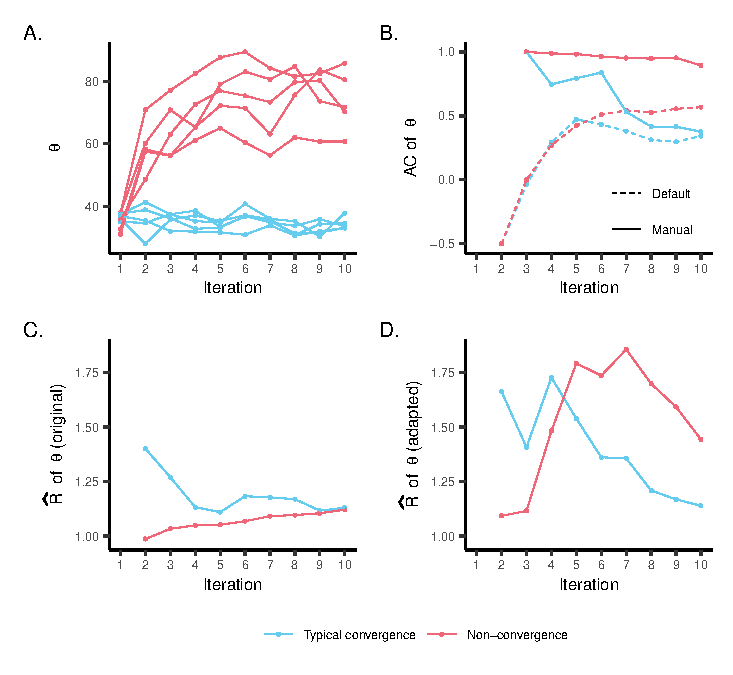
\includegraphics{2.Manuscript_files/figure-latex/diagnostics-1} 

}

\caption{Convergence diagnostics applied on the two scenarios from Figure 2 ($\theta$ = chain mean of variable $j$; $m=5$; $T=10$). Depicted are the imputation chains in panel A, two versions of the autocorrelation in panel B, and two versions of $\widehat{R}$ in panels C and D.}\label{fig:diagnostics}
\end{figure}

By visually inspecting the imputation chains in panel A, we conclude that the two scenarios show very different convergence. The typically converged algorithm initially portrays some signs of non-mixing (around \(t=2\)), but intermingles nicely overall. Additionally, there is very little trending in this scenario. The algorithm with pathological non-convergence shows severe non-mixing, although this gradually improves (beyond \(t=7\)). In this scenario, we see a lot of trending initially (up-to \(t=6\)), after which the chains reached a somewhat more stationary state.

When we look at panel B, we conclude something weird. The \(AC\)-values calculated with the default function indicate equal performance for the typical convergence and the pathological non-convergence scenarios (up-to \(t=5\)), while there is obvious trending in the \(\theta\)s of the latter. Moreover, the best convergence (as indicated by the lowest \(AC\)-value) is observed at \(t=2\) for both scenarios. However, if we look at the chain means of the non-convergence scenario, there should be signs of trending up-to iteration number seven. After consulting the documentation on \texttt{stats::acf()}, we conclude that this \(AC\) function is not suited for iterative imputation algorithms. The function is optimized for performance when \(t\geq50\) \citep{box15}, while the default number of iterations in iterative imputation is often much lower. Therefore, we compute \(AC\) manually (presented with solid lines in panel B). These \(AC\)-values behave as expected from visual inspection. We will, therefore, only consider manually calculated \(AC\)-values as non-convergence diagnostic.

In panel C, we do not see a lot of difference between the two scenarios either. The \(\widehat{R}\)-values are even somewhat lower for the non-convergence scenario than for the typical convergence. And apparently, the large variance causes an increase in \(\widehat{R}\)-values. Convergence seems to worsen with every additional iteration. This paints the wrong picture. An explanation for this behavior may be that under severe trending, the assumption of over-dispersion is violated. Taken together, this version of \(\widehat{R}\) is sub-optimal for assessing non-convergence in MI.

The \(\widehat{R}\)-values in panel D are conform our expectations. The adapted version of \(\widehat{R}\) depicted here does indicate less signs of non-convergence as the number of iterations goes up. An exception to this general trend is the `dip' around \(t=3\). As diagnostic tool, this may lead to the incorrect conclusion that the non-convergence scenario has superior convergence compared to the typical scenario. We can explain this as a downside of the low number of iterations in iterative imputation: the adapted version of \(\widehat{R}\) can only be completely employed if the number of iterations is at least four. Otherwise, it is not possible to perform all three transformations to the chains of \(\theta\)-values. For low values of \(t\), the \(\widehat{R}\)-values conform Vehtari et al.~are, therefore, more similar to the original \(\widehat{R}\) by Gelman and Rubin.

In short, both non-convergence diagnostics have a version that may be appropriate for iterative imputation algorithms. We will compute \(\widehat{R}\) conform \citet{veht19}, and calculate \(AC\) manually. The diagnostics will be applied to the four types of scalar summaries \(\theta\) described earlier: chain means, chain variances, a quantity of scientific interest, and the first eigenvalue of the variance-covariance matrix. We evaluate the performance of these eight sets of diagnostic methods (two diagnostics; four \(\theta\)s) through simulation.

\hypertarget{simulation-study}{%
\section{Simulation study}\label{simulation-study}}

The simulation study aims to determine to what extend non-convergence affects iterative imputation algorithms. Specifically, we are interested in the validity of inferences drawn from incomplete data using the MICE algorithm. And, whether invalid inferences due to non-convergence may be detected using eight sets of diagnostic methods. If the estimated quantities of scientific interest \(\bar{Q}\) are unbiased and confidence-valid estimates of \({Q}\), we will conclude that the algorithm is sufficiently converged for practical purposes. In contrast to this, we defined \emph{approximate} convergence as the most converged state that the algorithm can obtain. Continued iteration after reaching approximate convergence does not yield better mixing or stationarity (indicated by non-improving \(\widehat{R}\)- and \(AC\)-values). Continued iteration after obtaining valid inferences may lead to a more converged state of the algorithm, but not better estimates.

To induce non-convergence, we consider two sets of simulation conditions: `missingness' and `early stopping'. Missingness refers to the severity of the missing data problem, which we determine by the proportion of incomplete cases in dataset \(y\), \(p_{\rm inc}\). Early stopping is defined by the number of iterations in the imputation algorithm, \(T\).

The missingness conditions are chosen to reflect the difficulty of the missingness problem. The underlying assumption is that a low proportion of incomplete cases \(p_{\rm inc}\) leads to quick algorithmic convergence, since there is a lot of information in the observed data. A higher \(p_{\rm inc}\) yields slower convergence---unless there is so little information in \(y_{\rm obs}\) that this is outweighed by the random component in the imputation algorithm. Then, convergence to a stable but highly variable state may be reached instantly. Still, we expect that missingness conditions with higher \(p_{\rm inc}\) will result in more signs of non-convergence.

The assumption inherent to the early stopping conditions is that terminating the imputation algorithm too early causes non-convergence. Generally, the algorithm will not reach convergence if \(T=1\), because the imputed values in the first iteration (at \(t=1\)) depend on the starting values \citep[which are sampled randomly from the set of observed datapoints;][]{buur18}. As the number of iterations increases, the imputation chains should become independent of the initial values, until approximate convergence is reached (i.e., when an additional iteration does not lead to a more converged state). We expect that we can induce non-convergence by early stopping in at least those conditions where \(T\) is smaller than the default number of iterations in \texttt{mice}, \(T=5\) \citep{mice}.

\hypertarget{hypotheses}{%
\subsection{Hypotheses}\label{hypotheses}}

\begin{enumerate}
\def\labelenumi{\arabic{enumi}.}
\item
  We expect that simulation conditions with a high proportion of incomplete cases \(p_{\rm inc}\) and a low number of iterations \(T\) will more often result in biased, invalid estimates of the quantities of scientific interest \(Q\).
\item
  We hypothesize that \(\widehat{R}\) and \(AC\) will correctly identify signs of non-convergence in those simulation conditions where any \(\bar{Q}\) is \emph{not} an unbiased and confidence-valid estimate of \(Q\).
\item
  We hypothesize that the recommended thresholds to diagnose non-convergence with \(\widehat{R}\) (\(\widehat{R} > 1.2\), \(\widehat{R} > 1.1\), and \(\widehat{R} > 1.01\)) may be too stringent for iterative imputation applications. In an empirical study, where \(\widehat{R}\) was used to inform the required imputation chain length, it took as many as 50 iterations to overcome the conventional non-convergence threshold \(\widehat{R}>1.2\). Yet, scientific estimates were insensitive to continued iteration from \(t=5\) onward \citep{lace07}. We, therefore, suspect that \(\widehat{R}\) may over-estimate signs of non-convergence in iterative imputation algorithms, compared to the validity of estimates. In contrast to this, signs of non-convergence can be under-estimated by \(\widehat{R}\), in exceptional cases where the initial values of the algorithm are not appropriately over-dispersed \citep[p.~437]{broo98}. In \texttt{mice}, initial values are chosen randomly from the observed data, hence we cannot be certain of over-dispersion in the initial values. In practice, we do not expect this to cause problems for identifying non-convergence with \(\widehat{R}\).
\item
  We expect that high \(AC\)-values are implausible in iterative imputation algorithms with typical convergence. After only a few iterations, the randomness induced by the algorithm should effectively mitigate the risk of dependency within chains.
\item
  We further hypothesize that multivariate \(\theta\)s are better at detecting non-convergence than univariate \(\theta\)s.
\end{enumerate}

\hypertarget{set-up}{%
\subsection{Set-up}\label{set-up}}

We investigate non-convergence of the MICE algorithm through model-based simulation in \texttt{R} \citep[version 3.6.3;][]{R}. The number of simulation repetitions is 1000, and the simulation set-up is summarized in the pseudo-code below. The complete \texttt{R} script of the simulation study is available from \href{https://github.com/hanneoberman/MissingThePoint}{github.com/hanneoberman/MissingThePoint}.

\begin{verbatim}
# pseudo-code of simulation 
1. simulate data 
for (number of simulation runs from 1 to 1000)
 for (missingness proportions 5%, 25%, 50%, 75% and 95%)
  2. create missingness
  for (number of iterations from 1 to 100)
   3. impute missingness
   4. perform analysis of scientific interest
   5. compute non-convergence diagnostics 
   6. pool results across imputations
   7. compute performance measures
 8. combine outcomes of all missingness proportions
9. aggregate outcomes of all simulation runs 
\end{verbatim}

\hypertarget{data-generating-mechanism.}{%
\subsubsection{Data-generating mechanism.}\label{data-generating-mechanism.}}

In this study, sampling variance is not of interest. Therefore, a single complete dataset may serve as comparative truth in all simulation repetitions \citep{vink14}. The data-generating mechanism is a multivariate normal distribution, representing person-data on three predictor variables in a multiple linear regression problem. Let the predictor space be defined as
\[
\begin{aligned}
\begin{pmatrix}X_1\\
X_2\\
X_3
\end{pmatrix} \sim \mathcal{N}
\begin{bmatrix}
\begin{pmatrix}
12\\
3\\
0.5
\end{pmatrix}\!\!,
\begin{pmatrix}
4 & 4 & 1.8 \\
4 & 16 & 4.8\\
1.8 & 4.8 & 9
\end{pmatrix}
\end{bmatrix}\!\!\text{.}\\[2\jot]
\end{aligned}
\]
A finite population of \(N=1000\) is simulated using the \texttt{mvtnorm} package \citep{mvtnorm}. Subsequently, a fourth variable is constructed as outcome variable \(Y\). For each unit \(i = 1, 2,..., N\), let
\[
Y_i = 1 + 2X_{1i} +.5X_{2i} - X_{3i} + \epsilon_i ,
\]
where \(\epsilon \sim \mathcal{N}(0, 100)\). This results in a dataset \(y\), where \(y_{\rm mis} = \emptyset\). In other words, \(y\) contains the complete set of observations for all units \(i\) on all variables \(j\) (where \(j = Y, X_1, X_2, X_3\)). From the complete dataset we obtain the true values of the scientific estimands \(Q\).

\hypertarget{scientific-estimands.}{%
\subsubsection{Scientific estimands.}\label{scientific-estimands.}}

We consider four types of \(Q\)s that are often of interest in empirical research. Namely, two descriptive statistics: the mean \(\mu_j\) and standard deviation \(\sigma_j\) of each variable \(j\). We also consider the regression coefficients of the predictors: \(\beta_1\), \(\beta_2\), and \(\beta_3\) in regression equation
\[Y' = \beta_0 + \beta_1 X_1 + \beta_2 X_2 + \beta_3 X_3,\]
where \(Y'\) is the expected value of the outcome. The final estimand is the proportion of variance explained by the set of predictors: coefficient of determination \(r^2\) (note that lower case \(r\) is used to avoid confusion with non-convergence diagnostic \(\widehat{R}\)). The scientific estimands are estimated by \(\bar{Q}\) in each simulation condition.

\hypertarget{simulation-conditions.}{%
\subsubsection{Simulation conditions.}\label{simulation-conditions.}}

In each simulation repetition, we \emph{ampute} the complete dataset conform the missingness conditions. The proportion of incomplete cases \(p_{\rm inc}\) varies between 5\% and 95\%, in incremental steps (\(p_{\rm inc}\) = .05, .25, .50, .75, .95). We consider all possible univariate and multivariate patterns of missingness, conform a `missing completely at random' missingness mechanism \citep[MCAR;][]{rubin87}. I.e., the probability to be missing is the same for all \(N \times k\) cells in \(y\), conditional on \(p_{\rm inc}\). We use the `mice' package \citep[function \texttt{mice::ampute()};][]{mice} to obtain an incomplete dataset \{\(y_{\rm obs}, y_{\rm mis}\)\} for each of the five missingness conditions.

We impute the missing values in \{\(y_{\rm obs}, \dot y_{\rm mis}\)\} according to the early stopping conditions. That is, we vary the number of iterations in the imputation algorithm between one and one hundred (\(T = 1,2,.,100\)). All imputation procedures are performed using \texttt{mice} \citep[function \texttt{mice()};][]{mice}, with Bayesian linear regression imputation, and five imputation chains (\(m=5\)). This results in \(m=5\) sets of imputations for each of the one hundred early stopping conditions, \(\dot y_{\rm imp, \ell}\).

Subsequently, we obtain the completed data per imputation, \{\(y_{\rm obs}, \dot y_{\rm imp, \ell}\)\}, by combining the imputed data with the observed data \citep[function \texttt{mice::complete()};][]{mice}. We estimate univariate \(Q\)s directly from the completed data, by averaging across imputations to obtain \(\bar{Q}\). Estimates of multivariate \(Q\)s are obtained after performing multiple linear regression \citep[function \texttt{stats::lm()},][]{R}. We pool the resulting estimates, \(\hat{Q}_\ell\), into a single \(\bar{Q}\) conform \citet{vink14}.

\hypertarget{methods.}{%
\subsubsection{Methods.}\label{methods.}}

We consider eight sets of diagnostic methods to identify non-convergence, by applying \(\widehat{R}\) and \(AC\) on four different \(\theta\)s. Univariate \(\theta\)s are obtained from \(\dot y_{\rm imp, \ell}\). The model-independent multivariate \(\theta\), \(\lambda_{1}\), is obtained from \{\(y_{\rm obs}, \dot y_{\rm imp, \ell}\)\} as the variance in the first PCA component {[}function \texttt{stats::princomp}; R{]}. The model-dependent multivariate \(\theta\) is one of the quantities of scientific interest: the estimated regression coefficients in \{\(y_{\rm obs}, \dot y_{\rm imp, \ell}\)\}. We apply the two non-convergence diagnostics on the \(\theta\)s by implementing the adapted version of \(\widehat{R}\) and by manually programming the \(AC\) function.

\hypertarget{performance-measures.}{%
\subsubsection{Performance measures.}\label{performance-measures.}}

As recommended by \citet{buur18}, we evaluate the performance of the imputation algorithm with bias, coverage rate (CR), and confidence interval width (CIW). Bias is calculated for each \(Q\), whereas CR and CIW are only obtained for \(Q = \beta\). We calculate bias as \(\bar{Q} - Q\). CR is defined as the percentage of simulation repetitions in which the 95\% confidence interval (CI) around \(\bar{Q}\) covers the true estimand \(Q\). Let
\[\text{CI} = \bar{Q} \pm t_{(m-1)} \times \rm SE_{\bar{Q}},\]
where \(t_{(M-1)}\) is the quantile of a \(t\)-distribution with \(m-1\) degrees of freedom, and \(\rm SE_{\bar{Q}}\) is the square root of the pooled variance estimate. If we obtain nominal coverage (CR = 95\%), we can conclude that \(\bar{Q}\) is a confidence-valid estimate of \(Q\). Finally, we inspect CI width (CIW): the difference between the lower and upper bound of the 95\% confidence interval around \(\bar{Q}\). CIW is of interest because it is a measure of efficiency. Under nominal coverage, short CIs are preferred, since wider CIs indicate lower statistical power.

We evaluate the diagnostic methods to identify non-convergence against these performance measures. \(\widehat{R}\) and \(AC\) should identify non-convergence in simulation conditions, where \(\bar{Q}\) is \emph{not} an unbiased, confidence-valid estimate of \(Q\).

\hypertarget{results}{%
\section{Results}\label{results}}

Our results show the performance of the MICE algorithm under different conditions of missingness and early stopping. For reasons of brevity, we only discuss results for the worst-performing estimates in terms of bias. For univariate scientific estimands (\(Q=\mu\) and \(Q=\sigma\)) we observe the largest bias in the outcome variable \(Y\). And for the regression coefficients (\(Q=\beta\)) the bias is most pronounced in \(\beta_1\) (the effect of \(X_1\) on \(Y\)). Since there is just one estimate for \(Q=r^2\) to evaluate, we consider \(Q=\mu_Y, \sigma_Y,r^2, \beta_1\). In the figures, we present all missingness conditions, but only early stopping conditions where \(1 \leq T\leq50\). That is, the results are more or less stable for conditions where \(T \geq 30\). Full results are available from \href{https://github.com/hanneoberman/MissingThePoint}{github.com/hanneoberman/MissingThePoint}.

\hypertarget{quantities-of-scientific-interest}{%
\subsection{Quantities of scientific interest}\label{quantities-of-scientific-interest}}

\begin{figure}

{\centering 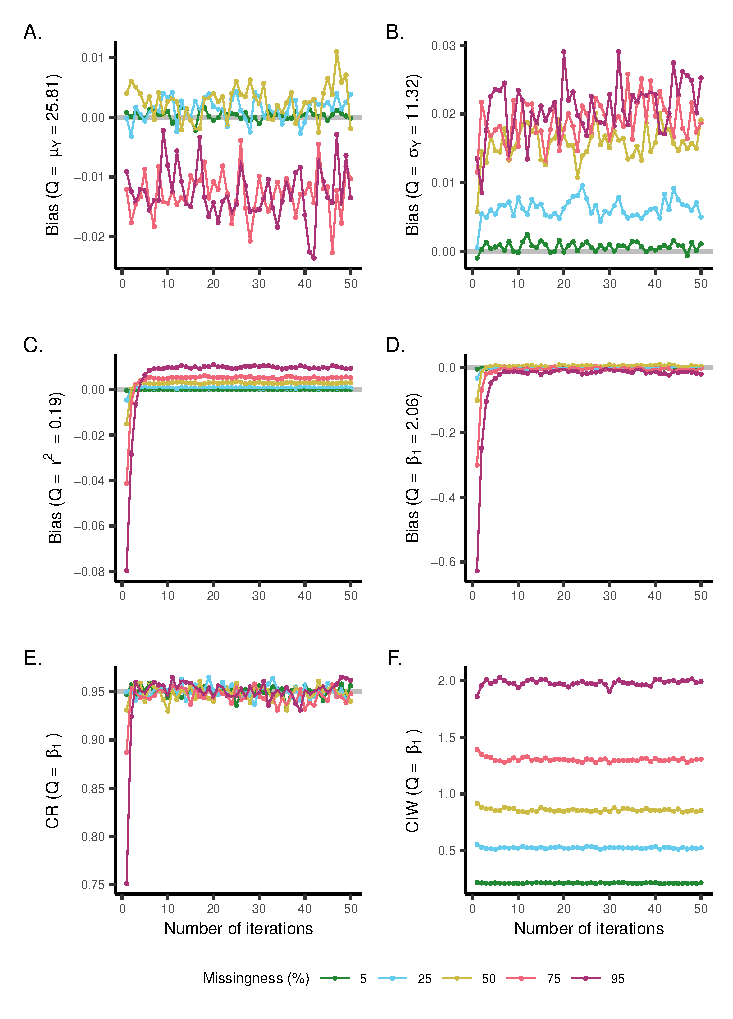
\includegraphics{2.Manuscript_files/figure-latex/Qs-1} 

}

\caption{Impact of non-convergence on statistical inferences. Depicted are the bias, coverage rate (CR) and confidence interval width (CIW) of the estimates $\bar{Q}$. We present the subset of $Q$s with the worst performance in terms of bias: the mean and standard deviation of $Y$, and the regression coefficient of $X_1$.}\label{fig:Qs}
\end{figure}

Figure \ref{fig:Qs} displays the influence of missingness and early stopping on the estimated quantities of scientific interest, \(Q\)s. In the first row of the figure, we see the bias in the estimated descriptive statistics (\(Q=\mu_Y\) and \(Q=\sigma_Y\); panels A and B). The second row shows the bias in the multivariate scientific estimands (\(Q=r^2\) and \(Q=\beta_1\); C and D). The third row consists of the coverage rate (CR) and confidence interval width (CIW) of the estimated regression coefficient (\(Q=\beta_1\); E and F).

\hypertarget{qmu.}{%
\subsubsection{\texorpdfstring{\(Q=\mu\).}{Q=\textbackslash mu.}}\label{qmu.}}

The estimated univariate means seem unaffected by early stopping. This implies that approximately unbiased estimates may be obtained with as little as one iteration (\(T \geq 1\)). The bias in \(\bar{Q}\) depends solely on the proportion of incomplete cases, with \(p_{\rm inc}\geq.75\) leading to more extreme biases than other conditions. Completely unbiased estimates are only obtained in conditions where \(p_{\rm inc}\leq.50\). This is curious since the MCAR missingness mechanism should yield unbiased univariate estimates without employing multiple imputation. Note however, that the magnitude of the bias in these conditions is small: \(\mu_Y\) is maximally under-estimated by 0.02 units, while the true value of \(\mu_Y\) is 25.81 (\(\sigma_Y = 11.32\)). We, therefore, conclude that non-convergence does not substantially impact the validity of the inferences for \(Q=\mu\).

\hypertarget{qsigma.}{%
\subsubsection{\texorpdfstring{\(Q=\sigma\).}{Q=\textbackslash sigma.}}\label{qsigma.}}

The estimated standard deviations are not substantially impacted by early stopping either. While the estimates for \(T=1\) are not equal to other conditions, the bias is actually \emph{less} severe than for \(T\geq2\). Therefore, no iteration at all is needed to obtain approximately unbiased estimates for \(Q=\sigma\). Completely unbiased estimates are only obtained in conditions where \(p_{\rm inc}=.05\). The other missingness conditions are impacted by non-convergence in the order of increasing \(p_{\rm inc}\). Similar to \(Q=\mu\), the magnitude of the bias in \(Q=\sigma\) is negligible. We, therefore, conclude that neither one of the univariate \(Q\)s is affected substantially by non-convergence.

\hypertarget{qr2.}{%
\subsubsection{\texorpdfstring{\(Q=r^2\).}{Q=r\^{}2.}}\label{qr2.}}

In contrast to the univariate estimates, the estimated coefficient of determination is clearly affected by early stopping, see Figure \ref{fig:Qs}C. The bias in \(Q\) appears to decrease with each additional iteration, while the magnitude of the bias still depends on the proportion of incomplete cases. Therefore, we see that the number of iterations that is necessary to reach stable, non-improving estimates also differs across missingness conditions. In conditions where \(p_{\rm inc}=.05\), estimates are unbiased after one iteration. The highest number of iterations necessary to reach approximate unbiasedness is seven (\(p_{\rm inc}=.95\); \(T\geq7\)). Completely unbiased estimates are only obtained in conditions where \(p_{\rm inc}\leq.25\). This implies that even for biased estimates, \(T\geq7\) would suffice to reach a stable solution.

\hypertarget{qbeta.}{%
\subsubsection{\texorpdfstring{\(Q=\beta\).}{Q=\textbackslash beta.}}\label{qbeta.}}

For the estimated regression coefficients, we first consider bias, before discussing CR and CIW. As Figure \ref{fig:Qs}D shows, the bias in \(\bar{Q}\) is affected by both the proportion of incomplete cases and the number of iterations. Similar to \(Q=r^2\), we observe approximately unbiased estimates after at least one, and at most seven iterations, depending on \(p_{\rm inc}\). Completely unbiased estimates are only obtained in conditions where \(T\geq3\) and \(p_{\rm inc}\leq .50\). Despite persistent bias in conditions where \(p_{\rm inc}\geq.75\), the coverage rates are non-improving after just three iterations, irrespective of \(p_{\rm inc}\). We conclude that any condition where \(T\geq3\) yields approximately nominal coverage rates, and thus confidence-valid estimates.
The nominal coverages can be explained by the CIWs. The CIWs depicted in Figure \ref{fig:Qs}F are conform the theoretical foundation of MI: CIs are wider in conditions with higher proportions of incomplete cases (i.e., there is less information in the data, and thus more uncertainty due to missingness). Since conditions with higher \(p_{\rm inc}\) result in both wider CIs and more severe bias, the true value of \(Q\) may be included in the CI, despite of the bias in \(\bar{Q}\).
We conclude that approximately unbiased estimates may be obtained in conditions where \(T\geq7\), whereas confidence-valid estimates require at most three iterations.

\hypertarget{summary.}{%
\subsubsection{Summary.}\label{summary.}}

These results demonstrate that the estimates of univariate scientific estimands \(Q\) are not impacted by early stopping of the MICE algorithm or the proportion of incomplete cases in \(y\). Unbiased estimates may be obtained after just one iteration. Multivariate estimates, by contrast, are affected by both the number of iterations and the proportion of missing cases. Completely unbiased estimates are only obtained under low to moderate missingness (\(p_{\rm inc}\leq.50\)), after at most three iterations. We observe approximately unbiased estimates after at most seven iterations (for any \(p_{\rm inc}\) considered). This implies that the algorithm produces stable, non-improving estimates when \(T\geq7\).

\hypertarget{non-convergence-diagnostics-1}{%
\subsection{Non-convergence diagnostics}\label{non-convergence-diagnostics-1}}

Figure \ref{fig:rhats-acs} displays results of the eight sets of diagnostic methods. The two columns in the figure represent the non-convergence diagnostics \(\widehat{R}\) and \(AC\); the rows depict the four scalar summaries \(\theta\) under consideration. The first row in Figure \ref{fig:rhats-acs} thus shows \(\widehat{R}\) and \(AC\) applied on the chain means (panels A and B). In the second row, we see the diagnostics applied on the chain variances (C and D). The third row depicts the same for \(\theta=\hat{Q}\) (E and F). And in the last row, we see the diagnostics applied on the novel \(\theta\) to consider: \(\lambda_1\) (G and H). We evaluate the performance of the methods by establishing whether they correctly identify conditions in which \(\bar{Q}\) is \emph{not} an unbiased, confidence-valid estimate of \(Q\). As we concluded in the last section, substantially biased estimates were only obtained in conditions where \(T\leq6\), and we observed non-nominal coverage only when \(T\leq3\). However, there was some persistent bias in conditions where \(p_{\rm inc}\geq.75\), irrespective of the number of iterations. If the diagnostic methods are appropriate for MI, we will detect non-convergence in these conditions.

\begin{figure}

{\centering 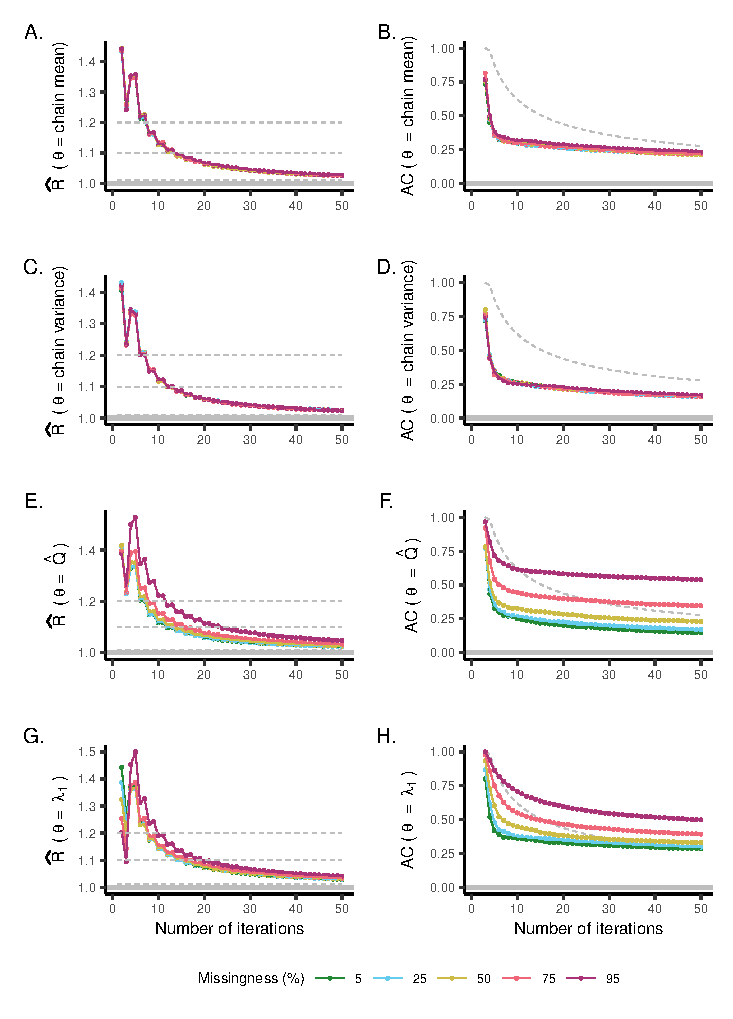
\includegraphics{2.Manuscript_files/figure-latex/rhats-acs-1} 

}

\caption{Non-convergence diagnostics $\widehat{R}$ and $AC$ applied on several $\theta$s. The left-hand side of the figure contains $\widehat{R}$-values, and the right-hand side contains $AC$-values. Depicted in the rows are the scalar summaries $\theta$: chain mean, chain variance, the quantity of scientific interest $\hat{Q}$, and the first eigenvalue of the variance-covariance matrix $\lambda_1$.}\label{fig:rhats-acs}
\end{figure}

\hypertarget{theta-chain-mean.}{%
\subsubsection{\texorpdfstring{\(\theta=\) chain mean.}{\textbackslash theta= chain mean.}}\label{theta-chain-mean.}}

As expected, \(\widehat{R}\) lowers with the number of iterations. After an initial `dip' in conditions where \(T=3\), we observe a gradual decrease in \(\widehat{R}\)-values with every additional iteration. This implies improving convergence, until the decrease tapers off after 30 to 40 iterations. Using the threshold \(\widehat{R}>1.2\), we diagnose non-convergence in conditions where \(T\leq7\), whereas the threshold 1.1 is exceeded when \(T\leq13\). The very strict threshold 1.01 is surpassed in all conditions \(T\leq100\) (not shown), and therefore not informative under the current specifications. With this set of methods, we fail to identify simulation conditions with persistent bias due to high missingness proportions.

Similarly, \(AC\) decreases with higher \(T\)s. \(AC\) indicates improving stationarity in conditions where \(T\leq6\). The \(AC\)-values do not exceed the threshold defined by statistical significance of the \(AC\)-values. Based on this threshold, we fail to diagnose non-convergence in any condition.

\hypertarget{theta-chain-variance.}{%
\subsubsection{\texorpdfstring{\(\theta=\) chain variance.}{\textbackslash theta= chain variance.}}\label{theta-chain-variance.}}

As panel C and D in Figure \ref{fig:rhats-acs} show, the results of this set of methods are highly similar to those with chain means as \(\theta\). This holds for both \(\widehat{R}\) and \(AC\). The only apparent difference is in the \(\widehat{R}\) threshold 1.1. Instead of diagnosing non-convergence in conditions where \(T\leq13\), we now diagnose this when \(T\leq11\). All other observations are equivalent.

\hypertarget{thetahatq.}{%
\subsubsection{\texorpdfstring{\(\theta=\hat{Q}\).}{\textbackslash theta=\textbackslash hat\{Q\}.}}\label{thetahatq.}}

The \(\widehat{R}\)-values in Figure \ref{fig:rhats-acs}E show a similar trend across iterations as we observed for chain means and chain variances. Only conditions with very high missingness proportions (\(p_{\rm inc}\geq.75\)) diverge from the earlier observations. The \(\widehat{R}\)-values in these conditions do not taper off after 30 to 40 iterations, but rather between 40 to 50 iterations. The highest number of iterations at which non-convergence is still diagnosed according to the thresholds are 11 for \(\widehat{R}>1.2\), 23 for \(\widehat{R}>1.1\), and 100 for \(\widehat{R}>1.01\) (not shown).

The \(AC\)-values also follow earlier observations, with the same exception as for \(\widehat{R}\) (when \(p_{\rm inc}\geq.75\)). To reach maximum stationarity, these conditions require at most seven iterations instead of five. Moreover, the \(AC\)-values in these conditions exceed the threshold to diagnose non-convergence. Interestingly, this only occurs after ten or even thirty iterations, while we would expect more signs of trending early in the iterations. Since the \(AC\)-values are not improving or worsening when \(T\geq7\), we conclude that non-convergence is incorrectly diagnosed based on the threshold.

\hypertarget{thetalambda_1.}{%
\subsubsection{\texorpdfstring{\(\theta=\lambda_{1}\).}{\textbackslash theta=\textbackslash lambda\_\{1\}.}}\label{thetalambda_1.}}

Once again, we observe \(\widehat{R}\)-values with a similar trend across iterations. For this \(\theta\), the results differ only in the most extreme missingness condition. When \(p_{\rm inc}=.95\), we diagnose non-convergence at \(T\leq9\) according to \(\widehat{R}>1.2\), \(T\leq19\) for \(\widehat{R}>1.1\), and 100 for \(\widehat{R}>1.01\) (not shown). The `dip' in \(\widehat{R}\)-values at \(T=3\) is even more pronounced than with other \(\theta\)s. Some \(\widehat{R}\)-values even overcome the threshold of 1.2. If we would terminate the algorithm at \(T=3\), we would incorrectly conclude that the algorithm reached approximate convergence, according to this threshold.

\(AC\)-values are systematically higher for this \(\theta\) than for other scalar summaries. The \(AC\)-values also taper off at a later point in the iterations. This suggests improving stationarity up-to ten, or even thirty iterations, depending on the missingness proportion. Using the threshold, we diagnose non-convergence at some point in all missingness conditions. However, this occurs only after reasonably decreasing \(AC\)-values are obtained---again suggesting that non-convergence is incorrectly diagnosed.

\hypertarget{summary.-1}{%
\subsubsection{Summary.}\label{summary.-1}}

Overall, the methods to diagnose non-convergence perform as expected: they indicate more signs of non-convergence in conditions with worse performance in terms of bias and confidence-validity. Under low to moderate missingness, it does not seem to matter on which \(\theta\) the non-convergence diagnostics are applied. If we look at complete unbiasedness, however, we notice that univariate \(\theta\)s fail to diagnose the persistent bias in conditions where \(p_{\rm inc}\geq.75\).

The number of iterations necessary to obtain approximately unbiased, confidence-valid estimates corresponds to the \(\widehat{R}\) threshold 1.2. The thresholds 1.1 and 1.01 seem too strict compared to the validity of the inferences. The threshold to diagnose significant \(AC\)-values does not appear to be appropriate in at least the current set-up, and perhaps in iterative imputation in general. A better heuristic to diagnose non-stationarity with \(AC\) may be through evaluation of the \(AC\)-values across iterations: If the values do not substantially decrease with \(T\), approximate stationarity may be concluded.

\hypertarget{discussion}{%
\section{Discussion}\label{discussion}}

Before drawing any further conclusions, let us first return to the hypotheses that we formulated for the simulation study.

\begin{enumerate}
\def\labelenumi{\arabic{enumi}.}
\item
  As hypothesized, biased, invalid estimates of quantities of scientific interest occurred more often in simulation conditions with a high proportion of incomplete cases \(p_{\rm inc}\) and a low number of iterations \(T\). However, this only holds for multivariate scientific estimands. Univariate \(Q\)s are not substantially impacted by early stopping.
\item
  Our results also support the hypothesis that \(\widehat{R}\) and \(AC\) would correctly identify signs of non-convergence. We observed higher \(\widehat{R}\) and \(AC\)-values in conditions where \(\bar{Q}\)s were biased, invalid estimates of \(Q\)s.
\item
  We hypothesized that the recommended thresholds to diagnose non-convergence with \(\widehat{R}\) would be too stringent for iterative imputation applications. This hypothesis is only partially supported. \(\widehat{R}\) indicated improving convergence until 30 to 40 iterations, while approximately unbiased, confidence-valid estimates were obtained after just seven iterations. This roughly corresponds to the threshold of 1.2. The more stringent threshold 1.1 seems plausible compared to the decrease in \(\widehat{R}\)-values across iterations. The most recent threshold 1.01 does indeed seem to over-estimate the signs of non-convergence.
\item
  The results of this simulation study do not support the hypothesis that high \(AC\)-values are implausible in iterative imputation algorithms with typical convergence. We expected that the randomness induced by the algorithm would effectively mitigate the risk of dependency within chains after a few iterations. In this study, however, we observed \(AC\)-values as high as theoretically possible (\(AC=1\)). The second part of the hypothesis is not refuted: the \(AC\)-values did decrease quickly as a function of \(T\).
\item
  Our final hypothesis was that multivariate \(\theta\)s would be better at detecting non-convergence than univariate \(\theta\)s. Multivariate \(\theta\)s did indeed show superior performance under certain conditions (e.g., multivariate \(Q\)s and extreme missingness proportions).
\end{enumerate}

\hypertarget{conclusion}{%
\subsection{Conclusion}\label{conclusion}}

We have shown that non-convergence in iterative imputation algorithms goes hand in hand with biased, invalid estimates---at least for the multivariate quantities of scientific interest considered in this study. Identifying non-convergence may be a crucial aspect of drawing valid statistical inferences from incomplete data. We concluded that the current practice of visually inspecting non-convergence through traceplots of univariate scalar summaries of the state-space of the algorithm does not suffice. We, therefore, considered eight sets of diagnostic methods to identify non-convergence: two non-convergence diagnostics (\(\widehat{R}\) and \(AC\)), two univariate \(\theta\)s, a model-dependent multivariate \(\theta\), and a novel, model-independent multivariate \(\theta\). Signs of non-convergence due to early stopping were identified with each of the methods. Bias due to high proportions of incomplete cases was only identified with multivariate \(\theta\)s.

Since we obtained approximately unbiased, confidence-valid estimates after at most seven iterations, we conclude that the \(\widehat{R}\) threshold 1.2 is the most appropriate diagnostic cut-off. The threshold to diagnose non-stationarity with \(AC\) does not seem to apply. However, some signs of non-convergence were detected in simulation conditions many more iterations. Under moderate missingness (\(p_{\rm inc}\leq.50\)) \(\widehat{R}\)-values decreased substantially until 30 to 40 iterations, which implies that mixing in the algorithm still improved with each additional iteration. \(AC\)-values only improved until about six iterations, suggesting minimal improvement in trending was obtained beyond \(T=6\) in the current simulation set-up.

The main finding of this study is that valid inferences may be obtained much quicker than approximate algorithmic convergence is reached. Under the current specifications, univariate \(Q\)s did not require algorithmic convergence at all. They are unbiased almost instantly after the algorithm is initiated. Approximately unbiased, confidence-valid estimates of multivariate \(Q\)s were obtained after a maximum of seven iterations. Continued iterations beyond \(T = 7\) did not yield better estimates.

\hypertarget{implications}{%
\subsection{Implications}\label{implications}}

Iterative imputation algorithms such as MICE are known to yield valid results under severe missingness. With this study, we have shown that valid inferences can also be obtained under a combination of severe missingness and early stopping. Based on our results, the traditional threshold of \(\widehat{R}> 1.2\) would be appropriate for diagnosing non-convergence in iterative imputation algorithms. This is, however, not in line with the recent recommendations by \citet{veht19} to lower the threshold to 1.01. The discrepancy between our conclusion and Vehtari et al.~may be explained by the nature of iterative imputation algorithms. In the limit, iterative imputation algorithms have the same characteristics as other MCMC algorithms. But, in imputation procedures, a part of the distribution is already determined by the observed data, whereas the entire distribution is unknown in many other MCMC applications. Since we combine a known distribution with an unknown distribution, valid estimates may be reached much sooner. Convergence may, therefore, be diagnosed at a less stringent threshold.

The threshold to diagnose non-convergence with \(AC\) does not seem appropriate at all in iterative imputation algorithms. A better diagnostic cut-off would be the number of iterations at which an additional iteration does not substantially decrease the \(AC\)-values. In practice, this implies that the default number of iterations in MICE is not sufficient. \(AC\) can only be computed if \(T\geq3\), while the current default in the \texttt{mice} package is five \citep{mice}. Identifying a reasonable decrease in the \(AC\)-values across iterations (an `elbow') requires more than three observations. We, therefore, suggest to increase the default number of iterations in MICE to ten. The computational cost of five additional iterations has become less of a burden since MICE was introduced \citeyearpar{mice}. Moreover, an increased number of iterations would grant the opportunity to exclude the first iterations from evaluation with \(\widehat{R}\). Excluding \(T\leq3\) provides empirical researchers with a less ambiguous heuristic to diagnose non-convergence, because we expect the initial `dip' in \(\widehat{R}\)-values to disappear.

\hypertarget{recommendations-for-empirical-researchers}{%
\subsection{Recommendations for empirical researchers}\label{recommendations-for-empirical-researchers}}

Based on our results, we formulate several recommendations for empirical researchers who employ iterative imputation to draw inferences from incomplete data. We suggest that non-convergence may still be evaluated visually, but in addition to inspecting univariate summaries of the state-space of the algorithm (\(\theta\)s, e.g., chain means), multivariate \(\theta\)s should be considered. We propose the following steps:

\begin{enumerate}
\def\labelenumi{\arabic{enumi}.}
\item
  First, check traceplots of the default \(\theta\)s (e.g., chain means and chain variances) for signs of pathological non-convergence. Adjust the imputation model if necessary.
\item
  Subsequently, decide which multivariate \(\theta\)s to track across iterations. The novel \(\theta\) that we propose in this study, \(\lambda_1\) is scientific model-independent and may thus always be employed. Alternatively, specify your own scalar summary of interest \citep[see e.g.,][]{buur18}. Monitor these \(\theta\)s through visual inspection, or using a non-convergence diagnostic.
\item
  Compute non-convergence diagnostics \(\widehat{R}\) and \(AC\). Do \emph{not} use the original implementation to calculate \(\widehat{R}\) \citep{gelm92}, or the \texttt{R} function \texttt{stats::acf()} to compute \(AC\) \citep{R}. Instead, calculate \(\widehat{R}\) conform \citet{veht19} and compute autocorrelations manually (see e.g., \href{https://github.com/hanneoberman/MissingThePoint}{github.com/hanneoberman/MissingThePoint}).
\item
  And finally, use the threshold \(\widehat{R}>1.2\) to diagnose non-mixing, and assess stationarity by plotting the autocorrelation over iterations. Keep iterating until the threshold for mixing is overcome, and until reasonably decreasing asymptotic \(AC\)-values are obtained. At that point, inferences are unlikely to improve by continued iteration.
\end{enumerate}

\hypertarget{limitations}{%
\subsection{Limitations}\label{limitations}}

Much remains unknown about non-convergence in iterative imputation algorithms. Even though we have demonstrated the appropriateness of \(\widehat{R}\) and \(AC\) as non-convergence diagnostics in this study, results may not extrapolate to other situations. In this study, we only considered the iterative imputation algorithm implemented in the \texttt{mice} package. The performance of the non-convergence diagnostics may depend on the characteristics of this specific algorithm. A potential threat to the ability to detect non-mixing with \(\widehat{R}\), for example, is the assumption of over-dispersed initial states. In \texttt{mice}, the algorithm is initiated by sampling starting values at random from the observed data, whereas other imputation software may use the average of the observed cases. The latter could lead to a systematical under-estimation of the variability in the first few iterations and violate the assumption of over-dispersion. In those cases, it would be more difficult to detect non-convergence with \(\widehat{R}\). Therefore, the diagnostic might not be appropriate outside of \texttt{mice}.

Moreover, the current simulation conditions were restricted to a single missingness mechanism. Proper performance under a `missing completely at random' (MCAR) mechanism is a necessary condition for any missing data method. It does not, however, guarantee equal performance under different missingness mechanisms. Future research should determine the performance of \(\widehat{R}\) and \(AC\) under `missing at random' and `missing not at random' mechanisms. Another parameter to consider in future research is the choice of the imputation method. As \citet{murr18} concluded, the behavior of algorithms such as MICE under certain default imputation models is still an open research question. We have investigated the behavior of MICE under only one type of model (Bayesian linear regression). Different imputations models might converge more poorly.

The imputation model may even be mis-specified on purpose, to induce non-convergence of different severity levels. Qualitatively, we have shown that \(\widehat{R}\) and \(AC\) are appropriate under clear violation of convergence. Quantitatively, we have only demonstrated that they can identify signs of non-convergence under MCAR, when the imputation model is a correctly specified Bayesian linear regression model. \newline \newline

\noindent In short, we have shown that iterative imputation algorithms can yield correct outcomes, even when a converged state has not yet formally been reached. Any further iterations would then burn computational resources without improving the statistical inferences. Our study found that---in the cases considered---inferential validity was achieved after five to ten iterations, much earlier than indicated by the \(\widehat{R}\) and AC diagnostics. Of course, it never hurts to iterate longer, but such calculations hardly bring added value.

\bibliographystyle{sageh}
\bibliography{thesis.bib}


\end{document}
